\scanpage{8}
% Upper-right mottled trace: visible patches only; no character, hand or role assigned.
\margin{
\begin{tikzpicture}[x=1cm,y=1cm]
\draw[gray,line width=.7pt] (.10,.84) -- (.29,.83) -- (.34,.78);
\fill[gray] (.08,.84) circle(.028cm);
\draw[gray,line width=.5pt] (.37,.70) -- (.38,.63) -- (.43,.56);
\draw[gray,line width=.45pt] (.20,.65) -- (.21,.59);
\draw[gray,line width=.45pt] (.27,.50) .. controls(.32,.45) and(.40,.46) .. (.43,.49);
\draw[gray,line width=.65pt] (.13,.31) .. controls(.19,.42) and(.29,.43) .. (.36,.40);
\fill[gray] (.43,.12) circle(.023cm);
\draw[gray,line width=.4pt] (.43,.12) .. controls(.48,.14) and(.49,.19) .. (.48,.23);
\end{tikzpicture}}
Suppose that $q\alpha-\alpha'\ne0$ then
\[
\begin{aligned}
(1)\ \Longrightarrow\quad &p\mid\sum_{i=1}^{q-1}C_q^i\,a^i b'^{\,q-i-1}+b'^{\,q-1}\\
\Longrightarrow\quad &p\mid q\,a^{q-1}\qquad\text{For }p\mid b'\ \text{and for }i\ne q-1\quad q-i-1\deleted{\ne0}>0
\end{aligned}
\]
now $p\mid b'$ and $b'\mid b^q$ thus $b'\mathrel{\underset{1}{\smile}}a$ thus $p\mathrel{\underset{1}{\smile}}a$

\deleted{thus if $\unsure{p\ne1|p\ne q}$}
\[
(1)\ \Longrightarrow\quad p\mid q\qquad\text{thus }\deleted{p=1\ \text{or }}p=q\quad(\text{if }q\alpha-\alpha'\ne0)
\]
Thus if $p\ne q$ \quad
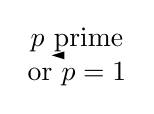
\begin{tikzpicture}[baseline=(p.base)]
\node[inner sep=0pt] (p) at (0,0) {$p$ prime};
\node[inner sep=0pt,anchor=north] at (0,-.28) {\inserted{or $p=1$}};
% Small dark triangular mark above the addition; its guiding function is uncertain.
\fill (-.32,-.20) -- (-.16,-.15) -- (-.16,-.25) -- cycle;
\end{tikzpicture}
and $p\mid b'$ then $\alpha'=q\alpha$
\begin{flushright}
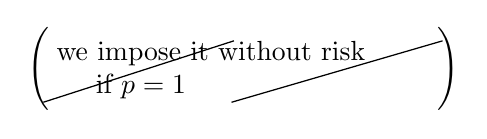
\begin{tikzpicture}[baseline=(u.base)]
\node[inner sep=0pt,anchor=west] (u) at (.22,0)
 {\rlap{we impose it without risk}\phantom{\deleted{we impose it without risk}}};
\node[inner sep=0pt,anchor=west] (v) at (.72,-.42)
 {\rlap{if $p=1$}\phantom{\deleted{if $p=1$}}};
\node[inner sep=0pt] at (0,-.20)
 {\rlap{$\Bigg($}\phantom{\deleted{$\Bigg($}}};
\node[inner sep=0pt] at (5.2,-.20)
 {\rlap{$\Bigg)$}\phantom{\deleted{$\Bigg)$}}};
% Two separate oblique cancellations over the two-line parenthesis.
\draw[line width=.45pt] (.06,-.62) -- (2.48,.16);
\draw[line width=.45pt] (2.45,-.62) -- (5.13,.16);
\end{tikzpicture}
\end{flushright}

Thus $\exists\,b_0\in\mathbb N^*$ and $\exists\,\gamma\in\mathbb N$ such that $b'=q^\gamma b_0^q$ \margin{$q\nmid b_0$}

moreover $b_0\mid b$ and if $b=b_0 b''$ then $b_0\mathrel{\underset{1}{\smile}}b''$ ?

Similarly $\exists\,a_0\in\mathbb N^*$ and $\exists\,\unsure{\zeta|\delta}\in\mathbb N$ such that $a'=q^\zeta a_0^q$ with $a_0\mid a$ and if $\overset{\unsure{\cdot|\prime}}{a}=a_0a''$ then $a_0\mathrel{\underset{1}{\smile}}a''$ ?

now $a\mathrel{\underset{1}{\smile}}b\Longrightarrow a_{\deleted{\unsure{0}}}'\mathrel{\underset{1}{\smile}}b'\Longrightarrow\zeta\times\gamma=0$ (and also $a_0\mathrel{\underset{1}{\smile}}b_0$)

I suppose henceforth that $\zeta=0$ thus $a'=a_0^q$

\figure{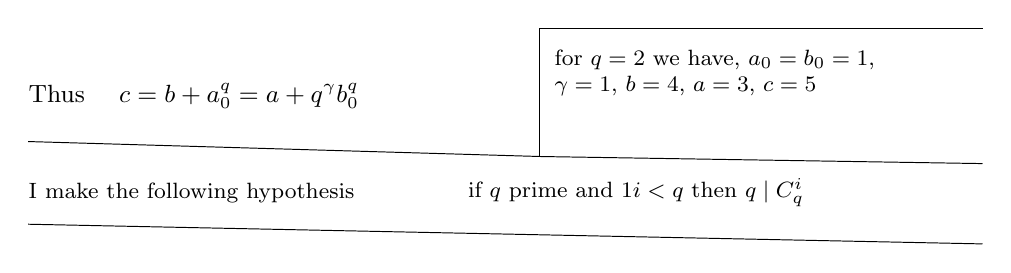
\begin{tikzpicture}[x=1cm,y=1cm]
\node[anchor=west,inner sep=0pt,font=\small] at (0,.80)
 {Thus \quad $c=b+a_0^q=a+q^\gamma b_0^q$};
\node[anchor=north west,inner sep=0pt,font=\footnotesize] at (6.68,1.43)
 {\begin{tabular}{@{}l@{}}
 for $q=2$ we have, $a_0=b_0=1$,\\
 $\gamma=1$, $b=4$, $a=3$, $c=5$
 \end{tabular}};
% Open right border; the left edge meets the shared long upper rule.
\draw[line width=.35pt] (12.12,1.66) -- (6.50,1.66) -- (6.50,.03);
\draw[line width=.35pt] (0,.22) -- (6.50,.03) -- (12.12,-.06);
\node[anchor=west,inner sep=0pt,font=\footnotesize] at (0,-.43)
 {I make the following hypothesis};
\node[anchor=west,inner sep=0pt,font=\footnotesize] at (5.58,-.43)
 {if $q$ prime and $1\leqslant i<q$ then $q\mid C_q^i$};
\draw[line width=.35pt] (0,-.83) -- (12.12,-1.08);
\end{tikzpicture}}
then If $q\geqslant3$ and $q\alpha-\alpha'\geqslant2$ \deleted{\unsure{then}} we have \inserted{$p=q,\ {\unsure{a|\alpha}}'=\gamma$}
\[
\begin{aligned}
(1)\ \Longrightarrow\quad
 &\deleted{\unsure{p^{2}|p}}q^2\mid q\,a^{q-1}\quad
 
\begin{tikzpicture}[baseline=(d.base)]
 \node[inner sep=0pt] (d) at (0,0)
  {\rlap{or $p=1$}\phantom{\deleted{or $p=1$}}};
 \draw[line width=.45pt] (d.west) -- (d.east)
  .. controls +(0.22,-.04) and +(0.22,-.06) ..
  ([yshift=-2pt]d.east) -- ([yshift=-2pt]d.west);
 \end{tikzpicture}
\quad
% Faint residual strokes and points in the interline gap; no character is supplied.
\begin{tikzpicture}[baseline=-.05cm,x=1cm,y=1cm]
\draw[gray,line width=.35pt] (0,.12) .. controls (.10,.02) and (.18,-.02) .. (.31,.02);
\draw[gray,line width=.35pt] (.21,.13) -- (.27,.10);
\draw[gray,line width=.35pt] (.34,.02) .. controls (.40,.17) and (.42,.26) .. (.52,.24);
\draw[gray,line width=.35pt] (.49,.15) -- (.64,.14);
\fill[gray] (.58,.31) circle (.5pt);
\fill[gray] (.64,.04) circle (.45pt);
\fill[gray] (.69,-.02) circle (.45pt);
\end{tikzpicture}\\[.8ex]
\Longrightarrow\quad
 &q\mid a^{q-1}\quad
 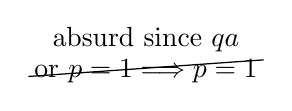
\begin{tikzpicture}[baseline=(d.base)]
 \node[inner sep=0pt] (d) at (0,0)
  {\rlap{or $p=1\Longrightarrow p=1$}\phantom{\deleted{or $p=1\Longrightarrow p=1$}}};
 \draw[line width=.45pt] ([xshift=-2pt,yshift=-2pt]d.west)
  -- ([xshift=2pt,yshift=4pt]d.east);
 \node[inner sep=0pt,anchor=south] at (0,.23)
  {\inserted{absurd since $q\nmid a$}};
 \end{tikzpicture}
\end{aligned}
\]
Thus $\gamma=0$ or $\gamma=$
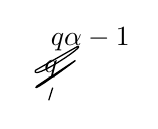
\begin{tikzpicture}[baseline=(q.base)]
\node[inner sep=0pt] (q) at (0,0)
 {\rlap{$q$}\phantom{\deleted{$q$}}};
% The live entry is physically raised above and to the right of the cancelled q.
\node[inner sep=0pt,anchor=south west] at (-.01,.22) {$q\alpha-1$};
\draw[line width=.45pt] (-.20,-.02) -- (.33,.28)
 .. controls (.48,.32) and (-.26,-.17) .. (-.20,-.02);
\draw[line width=.45pt] (-.18,-.22) -- (.30,.10)
 .. controls (.39,.16) and (-.29,-.34) .. (-.18,-.22);
\draw[line width=.45pt] (.02,-.24) -- (-.03,-.40);
\end{tikzpicture}
(provided that the hypothesis is true)%
\margin{\begin{tikzpicture}[baseline=(n.base)]
\node[inner sep=0pt,text width=.85\marginparwidth] (n)
 {This is perhaps interesting since here $2$ is set apart in
 \(\mathord{\overset{\scriptscriptstyle\unsure{/}}{\vphantom{l}}}\)the set of prime numbers};
% Small detached rising stroke before l'ensemble: role and hand unresolved.
% Return arrow rises at the right from the final parenthesis toward this note.
\fill ([xshift=.07cm,yshift=-.47cm]n.south east) circle(.022cm);
\draw ([xshift=.15cm,yshift=-.47cm]n.south east) -- ([xshift=.31cm,yshift=-.47cm]n.south east)
 -- ([xshift=.35cm,yshift=-.16cm]n.north east)
 .. controls([xshift=.35cm,yshift=-.03cm]n.north east) and([xshift=.19cm,yshift=-.01cm]n.north east)
 .. ([xshift=.06cm,yshift=.01cm]n.north east);
\draw ([xshift=.19cm,yshift=.14cm]n.north east) .. controls([xshift=.00cm,yshift=.04cm]n.north east) and([xshift=-.01cm,yshift=-.06cm]n.north east) .. ([xshift=.15cm,yshift=-.10cm]n.north east);
\end{tikzpicture}}
% archive sheet number: 7
